%%%%%%%%%%%%%%%%%%%%%%%%%%%%%%%%%%%%%%%%%%%%%%%%%%%%%%%%%%%%%%%%%%%%%
% LaTeX Template: Project Titlepage Modified (v 0.1) by rcx
%
% Original Source: http://www.howtotex.com
% Date: February 2014
% 
% This is a title page template which be used for articles & reports.
% 
% This is the modified version of the original Latex template from
% aforementioned website.
% 
%%%%%%%%%%%%%%%%%%%%%%%%%%%%%%%%%%%%%%%%%%%%%%%%%%%%%%%%%%%%%%%%%%%%%%

\documentclass[12pt]{report}
\usepackage[a4paper]{geometry}
\usepackage[myheadings]{fullpage}
\usepackage{fancyhdr}
\usepackage{lastpage}
\usepackage{graphicx, wrapfig, subcaption, setspace, booktabs}
\usepackage[T1]{fontenc}
\usepackage[font=small, labelfont=bf]{caption}
\usepackage{fourier}
\usepackage[protrusion=true, expansion=true]{microtype}
\usepackage[brazilian]{babel}
\usepackage{sectsty}
\usepackage{url, lipsum}
\usepackage[utf8]{inputenc}
\usepackage{indentfirst}
\usepackage{hyperref}
\usepackage{enumitem}
\usepackage{listings}
\usepackage{color}
\usepackage{xcolor}
\definecolor{lightgray}{rgb}{.9,.9,.9}
\definecolor{darkgray}{rgb}{.4,.4,.4}
\definecolor{purple}{rgb}{0.65, 0.12, 0.82}

\lstdefinelanguage{JavaScript}{
  keywords={typeof, new, true, false, catch, function, return, null, catch, switch, var, if, in, while, do, else, case, break},
  keywordstyle=\color{blue}\bfseries,
  ndkeywords={class, export, boolean, throw, implements, import, this},
  ndkeywordstyle=\color{darkgray}\bfseries,
  identifierstyle=\color{black},
  sensitive=false,
  comment=[l]{//},
  morecomment=[s]{/*}{*/},
  commentstyle=\color{purple}\ttfamily,
  stringstyle=\color{red}\ttfamily,
  morestring=[b]',
  morestring=[b]"
}

\lstset{
   language=JavaScript,
   backgroundcolor=\color{lightgray},
   extendedchars=true,
   basicstyle=\footnotesize\ttfamily,
   showstringspaces=false,
   showspaces=false,
   numbers=left,
   numberstyle=\footnotesize,
   numbersep=9pt,
   tabsize=2,
   breaklines=true,
   showtabs=false,
   captionpos=b
}

\colorlet{punct}{red!60!black}
\definecolor{background}{HTML}{EEEEEE}
\definecolor{delim}{RGB}{20,105,176}
\colorlet{numb}{magenta!60!black}
\lstdefinelanguage{json}{
    basicstyle=\normalfont\ttfamily,
    numbers=left,
    numberstyle=\scriptsize,
    stepnumber=1,
    numbersep=8pt,
    showstringspaces=false,
    breaklines=true,
    frame=lines,
    backgroundcolor=\color{background},
    literate=
     *{0}{{{\color{numb}0}}}{1}
      {1}{{{\color{numb}1}}}{1}
      {2}{{{\color{numb}2}}}{1}
      {3}{{{\color{numb}3}}}{1}
      {4}{{{\color{numb}4}}}{1}
      {5}{{{\color{numb}5}}}{1}
      {6}{{{\color{numb}6}}}{1}
      {7}{{{\color{numb}7}}}{1}
      {8}{{{\color{numb}8}}}{1}
      {9}{{{\color{numb}9}}}{1}
      {:}{{{\color{punct}{:}}}}{1}
      {,}{{{\color{punct}{,}}}}{1}
      {\{}{{{\color{delim}{\{}}}}{1}
      {\}}{{{\color{delim}{\}}}}}{1}
      {[}{{{\color{delim}{[}}}}{1}
      {]}{{{\color{delim}{]}}}}{1},
}


\newcommand{\HRule}[1]{\rule{\linewidth}{#1}}
\onehalfspacing
\setcounter{tocdepth}{5}
\setcounter{secnumdepth}{5}

%-------------------------------------------------------------------------------
% HEADER & FOOTER
%-------------------------------------------------------------------------------
\pagestyle{fancy}
\fancyhf{}
\setlength\headheight{15pt}
\fancyhead[L]{Michael Silva}
\fancyhead[R]{AnaclaraBot}
\fancyfoot[R]{Página \thepage\ de \pageref{LastPage}}
%-------------------------------------------------------------------------------
% TITLE PAGE
%-------------------------------------------------------------------------------

\begin{document}

\title{ \normalsize \textsc{1.0}
		\\ [2.0cm]
		\HRule{0.5pt} \\
		\LARGE \textbf{\uppercase{AnaclaraBot}}
		\HRule{2pt} \\ [0.5cm]
		\normalsize \today \vspace*{5\baselineskip}}

\date{}

\author{
		Michael Silva}

\maketitle
\tableofcontents
\newpage

%-------------------------------------------------------------------------------
% Section title formatting
\sectionfont{\scshape}


%-------------------------------------------------------------------------------

%-------------------------------------------------------------------------------
% BODY
%-------------------------------------------------------------------------------

\section*{Prefácio}
\addcontentsline{toc}{section}{Prefácio}
\setlength{\parindent}{10ex}

\par O objetivo deste documento é formalizar a arquitetura do software AnaclaraBot, como: as definições dos requisitos, funcionais e não funcionais, as tecnologias utilizadas em cada módulo do projeto e os métodos de desenvolvimento.
\\
\par Com esse documento, é possível entender todo o funcionamento do software em uma visão macro, no qual serão ilustrados os principais fluxos e transições. 


\newpage
\section*{Introdução}
\addcontentsline{toc}{section}{Introdução}
\setlength{\parindent}{10ex}

\par O AnaclaraBot é um software de conversação automatica, ou seja, não é necessário que uma pessoa esteja do outro lado para responder as perguntas de um internauta. Foi usada como base a tecnologia \emph{Watson} \hyperref[watson]{[1]} da IBM. A qual utiliza técnicas cognitivas, que ajudam na interpretação da linguagem natural fornecida pelo internauta, assim como na resposta que o sistema dará.

\par Então o administrador do sistema alimentará o \emph{Watson}, ligando prováveis respostas a palavras específicas. Com isso, o \emph{back-end} do AnaclaraBot irá consumir os serviços do \emph{Watson} passando como parâmetro o texto que o internauta enviar. Muitas vezes, existirá links contidos nos textos, os links são informações mais completas sobre determinado assunto.


\newpage
\section*{Descrição Geral do Sistema}
\addcontentsline{toc}{section}{Descrição Geral do Sistema}

\begin{enumerate}
\item \textbf{Problema:} Com o AnaclaraBot em pleno funcionamento, a empresa poderá reduzir os gastos de pessoal drasticamente. Já que, não será necessário uma equipe de telemarketing para se comunicar com os clientes, salvo em situações bastante específicas. O AnaclaraBot responderá e interpretará as interações com o cliente usando linguagem natural. É muito importante que o administrador do sistema alimente o \emph{Watson} corretamente, abrangindo os assuntos mais importantes, cujo os clientes necessitam de respostas ou informações.

\item \textbf{Regras de Negócio:} A versão do \emph{front-end} assim como \emph{back-end} será colocada em um servidor de ultravelocidade, o qual utiliza a tecnologia de \emph{cloud / elastic}, fornecido pela empresa \emph{Amazon}. Além dos arquivos de código do software, o BD (Banco de Dados) estará também nesse servidor. Toda a responsabilidade de tolerância a falhas e segurança de armazenamento das informações são de responsabilidade da mantenendora do servidor (\emph{Amazon}).

\item \textbf{Usuários do Sistema:} O sistema contempla basicamente 2 usuários: O \underline{Adminsitrador}, o qual alimenta/treina o \emph{Watson} e o \underline{Internauta} que interage com o \emph{Watson}, já treinado.

\item \textbf{Armazenamento:} Todas as conversas entre os internautas e o \emph{Watson} são persistidas em um banco de dados. Esses dados, posteriormente, poderão ser usados por alguma ferramenta de \emph{Business Intelligence } para que gere alguma informação relevante para a empresa.

\item \textbf{Desenvolvimento:} O desenvolvimento do software segue o padrão MVC, tanto o \textit{front-end} com o AngularJs (\underline{View:} Layout da aplicação;  \underline{Controller:} Chamadas a api's; \underline{Model: } Modelos dos objetos a serem enviados nas api's. ), quanto o \textit{back-end} com o NodeJs (\underline{View: } Especificação das api's; \underline{Controller:} Lógica de armazenamento no banco; \underline{Model: } Modelo MongoDB para salvar o objeto ).
\end{enumerate}




\newpage
\section*{Requisitos}
\addcontentsline{toc}{section}{Requisitos}


\begin{enumerate}
\item \textbf{Funcionais} O software AnaclaraBot será incluido no site de uma empresa, com isso, quando algum internauta acessar esse site, poderá iniciar uma conversa. A cada frase que esse internauta enviar, ela responderá conforme a identificação das palavras chaves contidas no texto (a acertude das respostas é de total responsabilidade do \textit{Watson}, juntamente com o treinamento que o administrador do sistema forneceu). A cada interação, as motivadas pelo internauta ou as respondidas pela AnaclaraBot serão armazenadas em um Banco de Dados. A descrição está na Figura \ref{fig:ana}.
\\
\\
\begin{figure}[!ht]
  \centering
      \includegraphics[width=0.92\textwidth]{AnaclaraBot}
  \caption{Descrição de funcionament}
  \label{fig:ana}
\end{figure}


\item \textbf{Não Funcionais} 
\begin{enumerate}
\item O \textit{back-end} estará disponível para as requisições dos internautas, assim como para armazenar as interações, desde que o servidor fornecido por terceiros \textit{Amazon} esteja em pleno funcionamento.

\item Terá uma senha, para que os seus serviços sejam consumidos, essa senha será armazenada em variável de ambiente do sistema operacional.

\item Somente os administradores do sistema terão as senhas de acesso ao servidor.

\item O software será desenvolvido seguindo os padrões de projetos descrita em \hyperref[designpat]{[2]}.

\item O software será desenvolvido para rodar na seguinte configração mínima: 1 CPU, Linux Ubuntu, 2GB de Memória Ram e Acesso a rede internet. Instância T2 Small da \textit{Amazon} \hyperref[amazon]{[3]}.

\item O sistema deverá ser acessado completamente via browser HTTP/HTML e via dispositivos Mobile.

\end{enumerate}


\end{enumerate}

\section*{Cronograma de Desenvolvimento}
\addcontentsline{toc}{section}{Cronograma de Desenvolvimento}


\begin{center}
\captionof{table}{Cronograma de Desenvolvimento da AnaclaraBot} \label{tab:title} 
\begin{tabular}{ |c|c|c|c| } 
\hline
1 & Pagamento Inicial: R\$ 366,00. & 21/10/2016 &  \\ \hline
2 & Arquitetura do Projeto & 24/10/2016 &  \\ \hline
3 & Arquitetura do Banco de Dados & 26/10/2016 &  \\ \hline
4 & Criação das API's & 31/10/2016 & Pagamento da parcela número 2. \\ \hline
5 & Persistência do JSON & 02/11/2016 &  \\ \hline
6 & Design do Front-End em imagem & 05/11/2016 & Pagamento da parcela número 3. \\ \hline
7 & Codificação do Front-End & 09/11/2016 & Pagamento da parcela número 4. \\ \hline
8 & Criar interface para trocar foto da atendente & 14/11/2016 &  \\ \hline
9 & Conectar o Front-End no Back-End & 14/11/2016 & Pagamento da parcela número 5. \\ \hline
\end{tabular}
\end{center}


\newpage
\section*{Tecnologias a serem utilizadas}
\addcontentsline{toc}{section}{Tecnologias a serem utilizadas}


\begin{enumerate}
\item \textbf{Back-End:} Foi utilizado o NodeJs \hyperref[nodejs]{[4]}.
\item \textbf{Front-End:} Foi utilizado HTML5, CSS3, jQuery, AngularJS, JS e Express \hyperref[express]{[5]}.
\item \textbf{Documentação das Api's:} Todas as API's produzidas pelo \textit{back-end} estão documentadas com o Swagger \hyperref[swagger]{[6]}.
\item \textbf{Layout:} O layout foi desenhado com o Adobe Photoshop \hyperref[ps]{[7]}.
\item \textbf{Banco de Dados:} O banco de dados foi desenvolvido com o MongoDB \hyperref[mongodb]{[8]}.

\end{enumerate}

\section*{Encapsulamento}
\addcontentsline{toc}{section}{Encapsulamento}

O Software tem duas partes integrantes e plugáveis, o \textit{back-end} e o \textit{front-end}. Ambas as partes podem funcionar separadamente, exercendo seus papéis, ou seja, pode ser conectado outro \textit{front-end} ao \textit{back-end} existente, e vice versa. Desde que siga a arquitetura planejada.

\par O \textit{back-end} pode servir várias instâncias de \textit{fron-end}, estando nos mesmos servidores ou não. Isso tem a idéia de containers, é altamente recomendado instalá-lo em um servidor com estrutura \textit{cloud}, o qual seus recursos de hardware e conexão crescem de acordo com a demanda.

\par É válido ressaltar que podemos separar cada parte do Software em containers, sendo o BD um container, o \textit{back-end} outro, por último, o \textit{fron-end}. Podem ficar em servidores separados (recomendado) ou no mesmo servidor (não é recomendado). Conforme a Figura \ref{fig:arc}.

\begin{figure}[!ht]
  \centering
      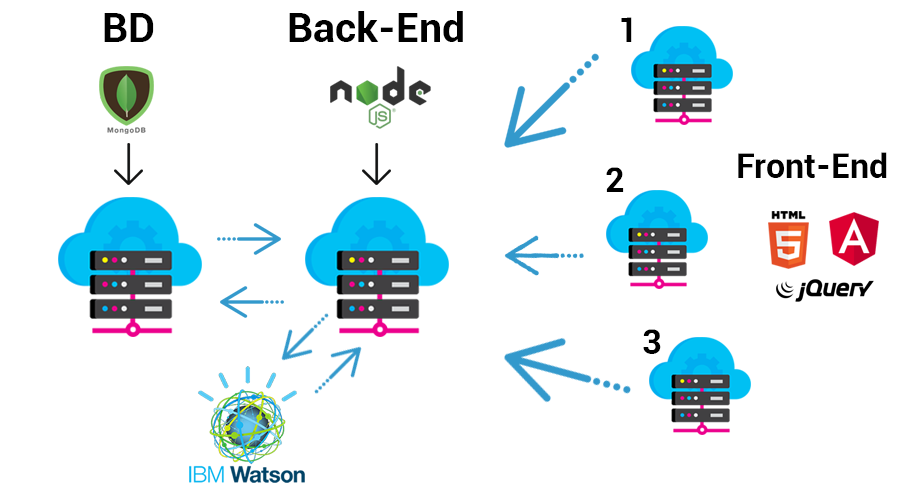
\includegraphics[width=0.55\textwidth]{arc}
  \caption{Arquitetura do Software}
  \label{fig:arc}
\end{figure}


\newpage
\section*{Arquitetura do Banco de Dados}
\addcontentsline{toc}{section}{Arquitetura do Banco de Dados}
\setlength{\parindent}{10ex}


O Banco de Dados do AnaclaraBot tem 3 coleções, são elas:
\begin{enumerate}

\item \textbf{User:} Contém os dados dos usuários que se cadastraram, e as referências para as conversas (\emph{Conversations}), as quais ele participou.

\item \textbf{Conversation:} Contém os meta-dados das conversas, referências para as interações (\emph{Interactions}) e um ou vários \textit{quizzes} que o usuário responde ao final do chat.

\item \textbf{Interaction:} Contém a pergunta do usuário, resposta do bot, os \textit{intents} e as \textit{entities}. Tanto a pergunta do usuário quanto a resposta do bot podem ser em formato de texto, áudio ou imagem.

\end{enumerate}


\par O modelo do Banco de Dados está descrito na Figura \ref{fig:diagram}.
\begin{figure}[!ht]
  \centering
      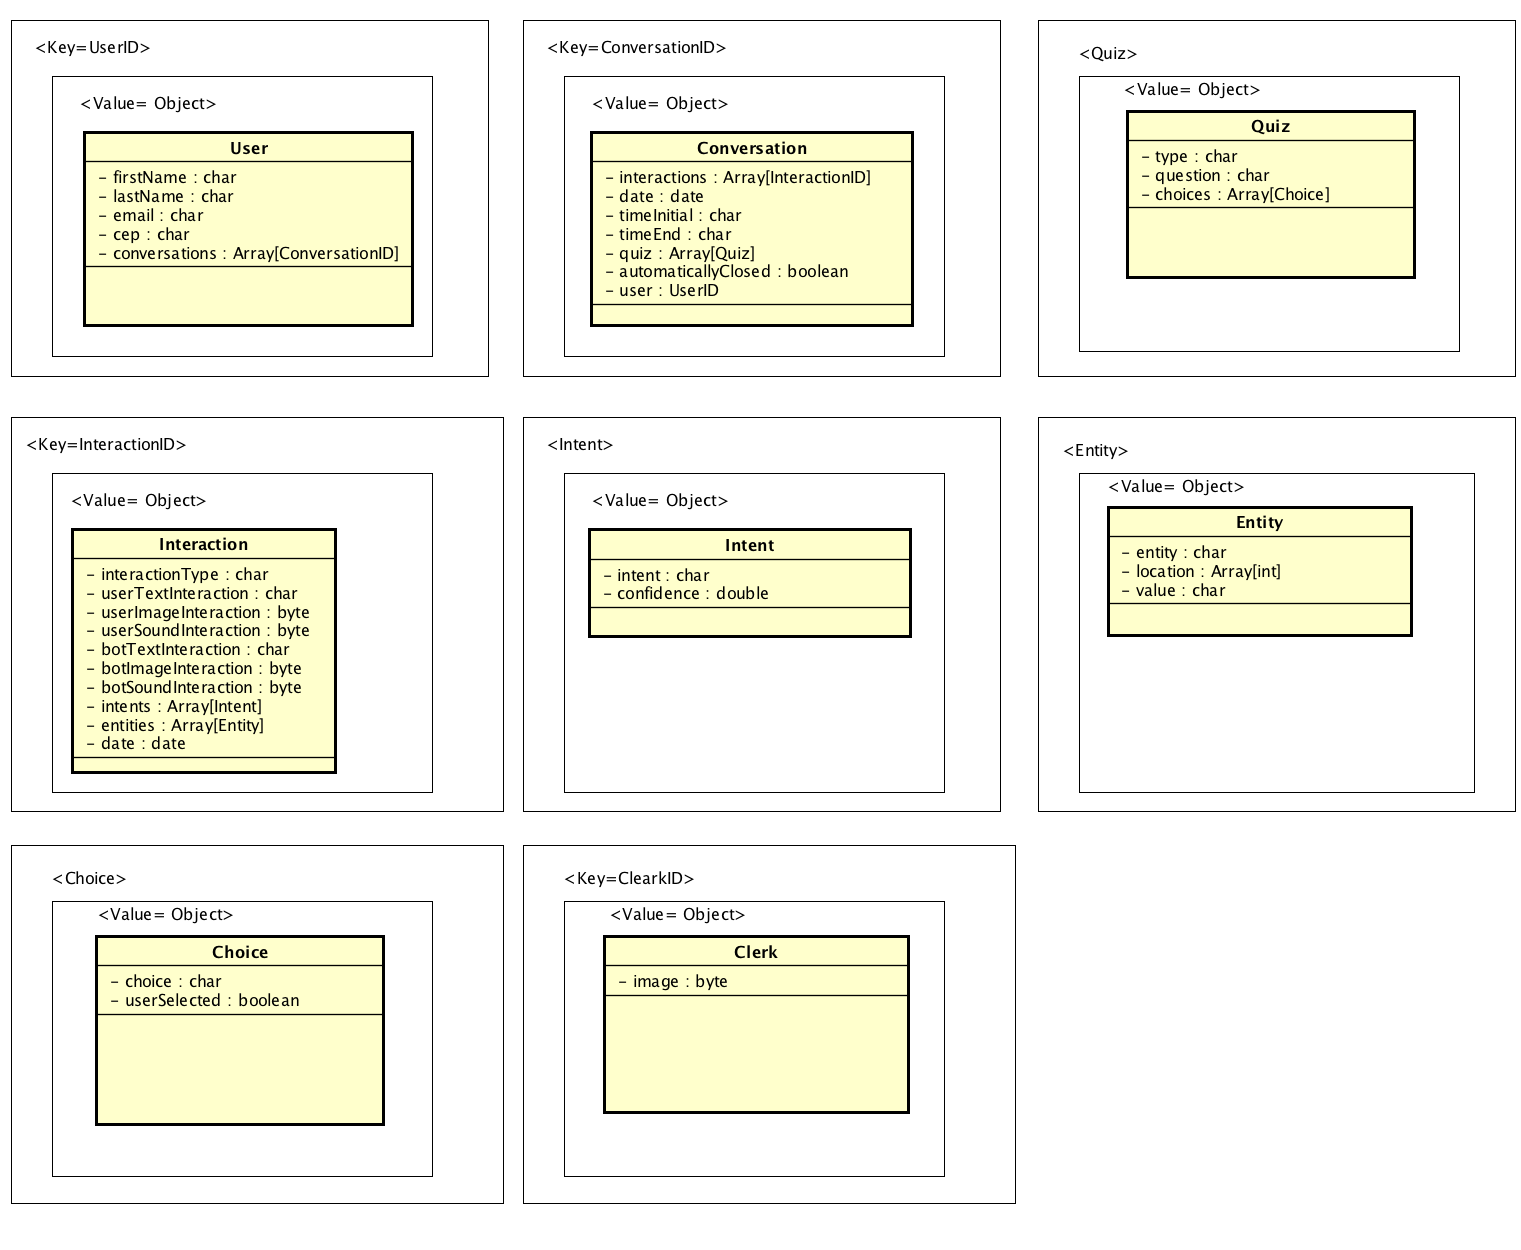
\includegraphics[width=0.9\textwidth]{diagram}
  \caption{Modelo do Banco de Dados}
  \label{fig:diagram}
\end{figure}


\newpage
\par Os exemplos da estrutura no formato MongoDB estão descrito nas Listings \ref{list:UserJsonSample}, \ref{list:ConversationJsonSample} e \ref{list:InteractionJsonSample}


\medskip
\begin{lstlisting}[language=json, caption= Exemplo da estrutura User de dados já no formato MongoDB, label={list:UserJsonSample}]
{
	"userId" 			: 1,
	"firstName" 		: "Luiz",
	"lastName"  		: "Medeiros",
	"email"				: "luiz.medeiros@cognitivesolutions.com.br",
	"cep"				: "72000-000",
	"conversations"		: ["12329-asdasd21-asdaad", "kopsa-09877-asd-asdad"]
}
\end{lstlisting}

\medskip
\begin{lstlisting}[language=json, caption= Exemplo da estrutura Conversation de dados já no formato MongoDB, label={list:ConversationJsonSample}]
{
	"conversationId" 		: "862c31dc-f06a-461d-860c-e36290c0b6e6",
	"date"		 			: "2016-10-06",
	"timeInitial"  			: "08:00:27",
	"timeEnd"				: "08:13:54",
	"automaticallyClosed"	: true,
	"user"					: 8372163732467,
	"interactions"			: [231231,937283,1231212],
	"quiz"					: [
							{
								"type"			: "multiple",
								"question"		: "Quais seus dias da semana preferidos?",
								"choices"		: [
									{
										"choice" 		: "Segunda",
										"userSelected"	: false
									},
									{
										"choice" 		: "Terça",
										"userSelected"	: true
									},
									{
										"choice" 		: "Quarta",
										"userSelected"	: true
									},
									{
										"choice" 		: "Quinta",
										"userSelected"	: true
									}
								]
							}, 
							{
								"type": "binary",
								"question"		: "Você gostou do atendimento?",
								"choices"		: [
									{
										"choice" 		: "Sim",
										"userSelected"	: false
									},
									{
										"choice" 		: "Não",
										"userSelected"	: false
									},
									{
										"choice" 		: "Não sei",
										"userSelected"	: true
									}
								]
							}
						  ]
}

\end{lstlisting}

\newpage
\medskip
\begin{lstlisting}[language=json, caption= Exemplo da estrutura Interaction de dados já no formato MongoDB, label={list:InteractionJsonSample}]
{
	"interactionId" 		: 2131,
	"userTextInteraction" 	: "vacina",
	"userImageInteraction"	: null,
	"userSoundInteraction"	: null,
	"botInteraction"  		: "Sempre mantenha [...]",
	"botImageInteraction"	: null,
	"botSoundInteraction"	: null,
	"date"					: "2016-11-02T16:29:09.000Z",
	"intents"				: [
								{
									"intent" 		: "Aeroporto",
									"confidence"	: "0.16709978332713935"
								},
								{
									"intent" 		: "vacinação",
									"confidence"	: "1"
								}
							  ],
	"entities"				: [
								{
									"entity" 		: "Aeroporto",
									"location"		: [0,4],
									"value"			: "mala"
								},
								{
									"entity" 		: "vacinação",
									"location"		: [0,6],
									"value"			: "cartão de vacinação"
								}
							  ]
}

\end{lstlisting}

\newpage
\section*{Script de criação do Banco de Dados}
\addcontentsline{toc}{section}{Script de criação do Banco de Dados}
\setlength{\parindent}{10ex}


\medskip
\begin{lstlisting}[caption= User Collection]
var UserSchema   = new mongoose.Schema({
    firstName: String,
    lastName: String,
    email: String,
    cep: String,
    conversations: [String]
});
\end{lstlisting}

\medskip
\begin{lstlisting}[caption= Interaction Collection]
var EntitySchema   = new mongoose.Schema({
    entity: String,
    location: [Number],
    value: String
});


var IntentSchema   = new mongoose.Schema({
    intent: String,
    confidence: Number
});


var InteractionSchema   = new mongoose.Schema({
    interactionType: String,
    userTextInteraction: String,
    userImageInteraction: Buffer,
    userSoundInteraction: Buffer,
    botTextInteraction: String,
    botImageInteraction: Buffer,
    botSoundInteraction: Buffer,
    date: String,
    intents: [IntentSchema],
    entities: [EntitySchema]
});

\end{lstlisting}

\newpage
\medskip
\begin{lstlisting}[caption= Conversation Collection]
var ChoiceSchema    = new mongoose.Schema({
    choice: String,
    userSelected: Boolean
});


var QuizSchema    = new mongoose.Schema({
    type: String,
    question: String,
    choices: [ChoiceSchema]
});

var ConversationSchema   = new mongoose.Schema({
    conversation_id: String,
    date: String,
    timeInitial: String,
    timeEnd: String,
    automaticallyClosed: Boolean,
    interactions: [{
        type: mongoose.Schema.Types.ObjectId,
        ref: 'Interaction'
    }],
    user: {
        type: mongoose.Schema.Types.ObjectId,
        ref: 'User'
    },
    quiz: [QuizSchema]
});

\end{lstlisting}

\medskip
\begin{lstlisting}[caption= Clerk Collection]
var ClerkSchema   = new mongoose.Schema({
    image: { data: Buffer, contentType: String }
});
\end{lstlisting}

\newpage
\section*{AnaclaraBot em imagens}
\addcontentsline{toc}{section}{AnaclaraBot em imagens}
\setlength{\parindent}{10ex}

\par Chat em minimizado em dispositivo mobile [\ref{fig:min_iphone}].
\begin{figure}[!ht]
  \centering
      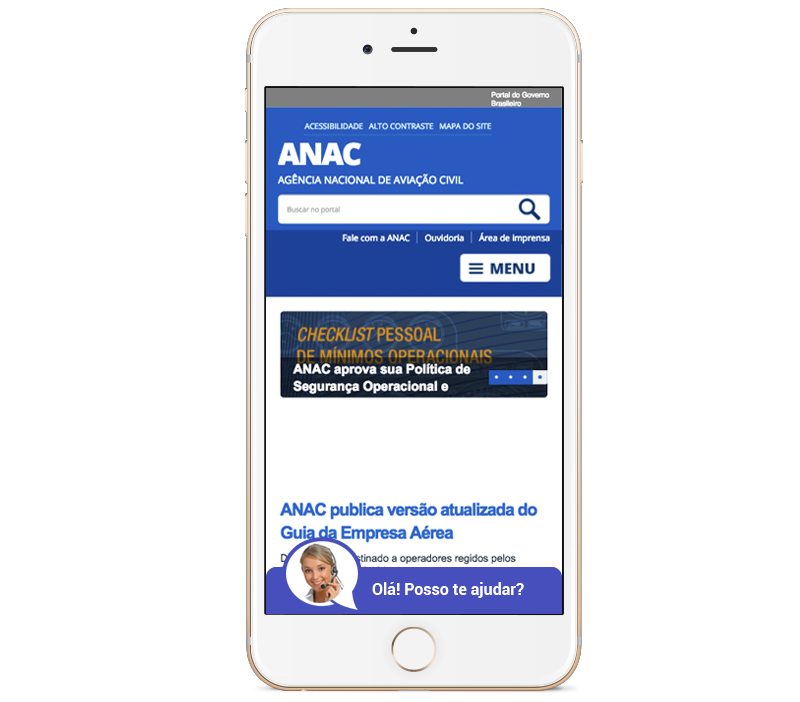
\includegraphics[width=0.9\textwidth]{front_chat_iphone_min}
  \caption{Minimizado em mobile}
  \label{fig:min_iphone}
\end{figure}

\newpage

\par Cadastramento de usuários em desktop.[\ref{fig:anac_cad}].
\begin{figure}[!ht]
  \centering
      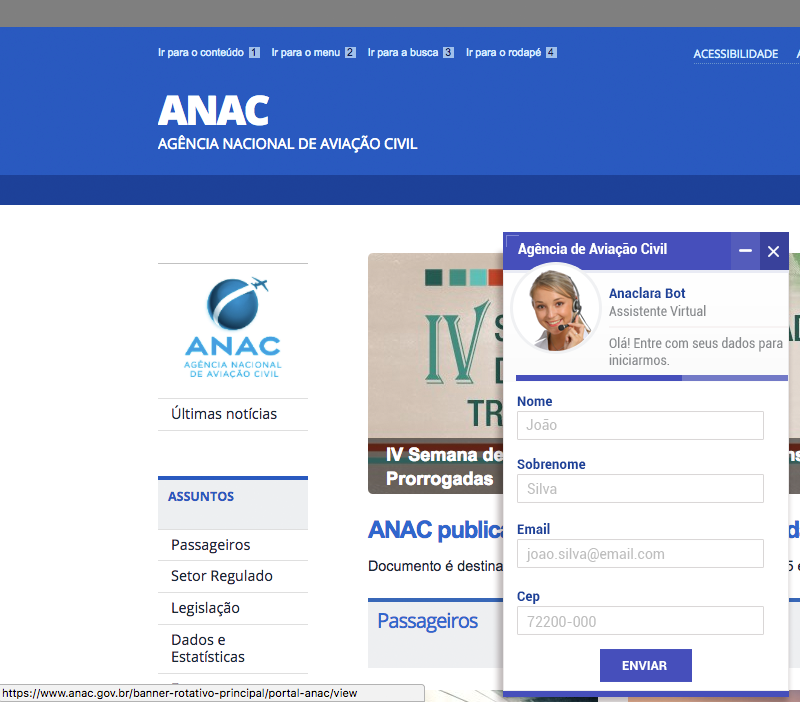
\includegraphics[width=0.9\textwidth]{no_site_anac_cad}
  \caption{Área de cadastro}
  \label{fig:anac_cad}
\end{figure}

\newpage

\par Área de conversasão em um site de exemplo.[\ref{fig:conversasao}].
\begin{figure}[!ht]
  \centering
      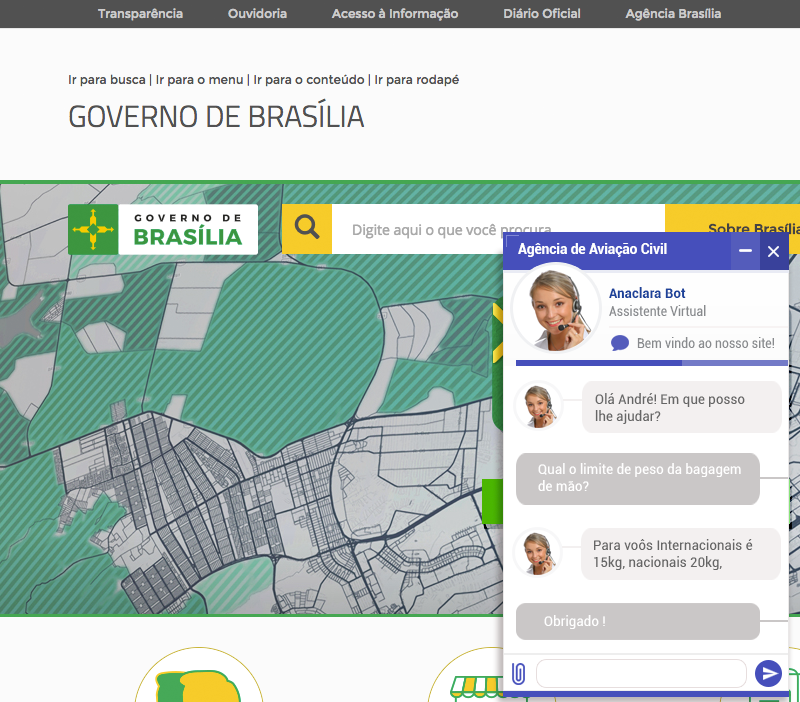
\includegraphics[width=0.9\textwidth]{no_site_gdf}
  \caption{Área de conversasão}
  \label{fig:conversasao}
\end{figure}

\newpage

\par Área de login para administrador.[\ref{fig:admin_login}].
\begin{figure}[!ht]
  \centering
      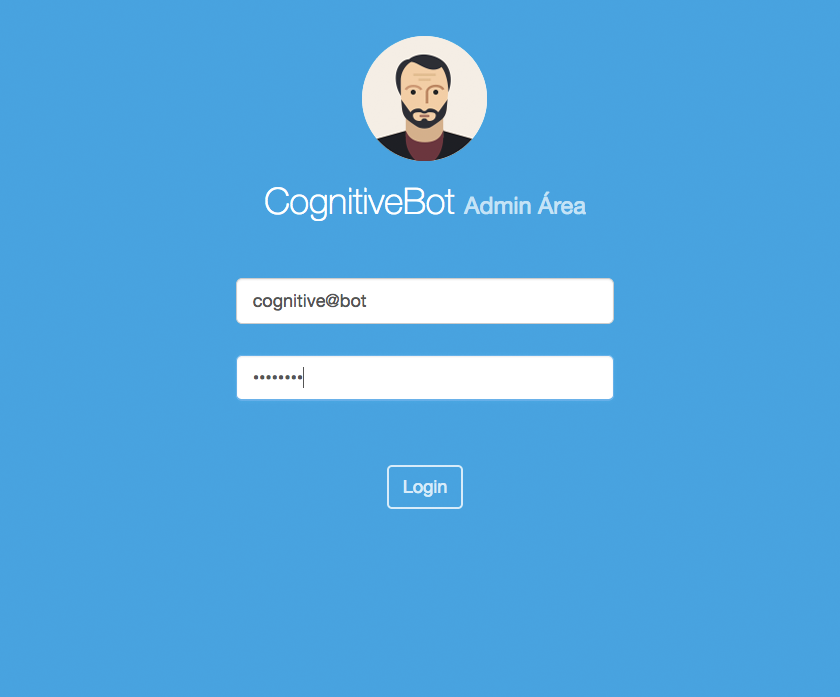
\includegraphics[width=0.9\textwidth]{admin_login}
  \caption{Área de login para administrador}
  \label{fig:admin_login}
\end{figure}

\newpage

\par Área de administrador, as informações podem ser alteradas..[\ref{fig:admin_info}].
\begin{figure}[!ht]
  \centering
      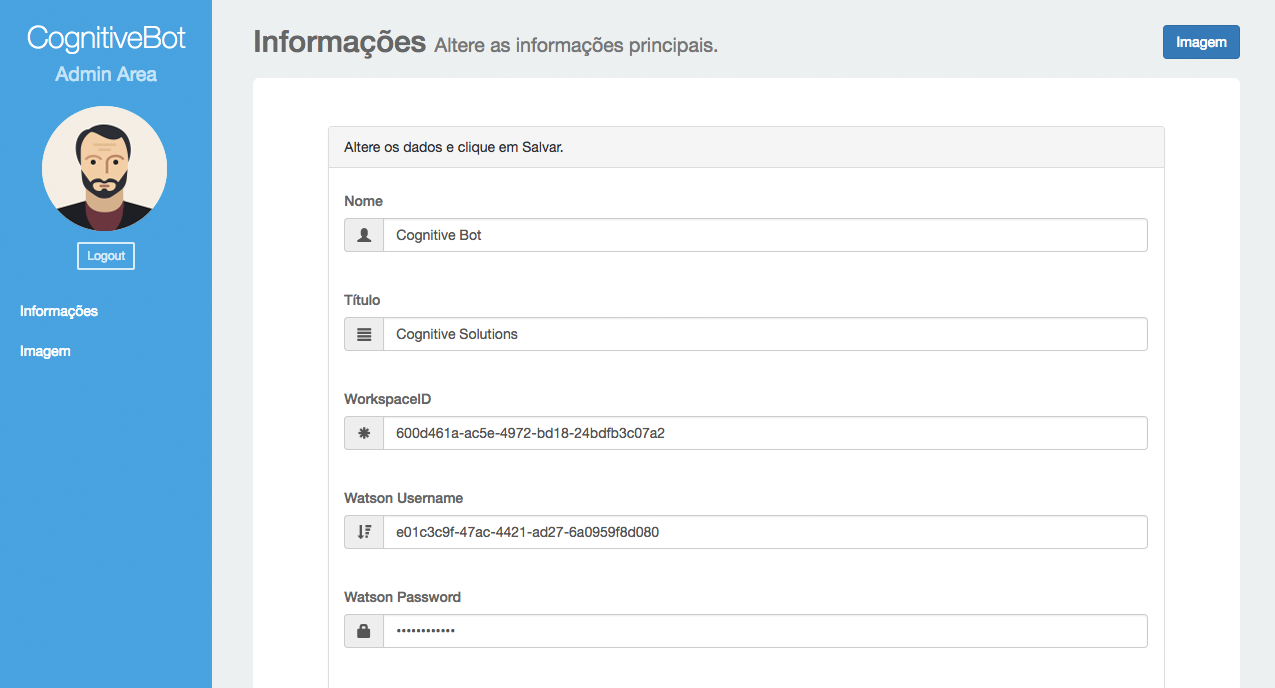
\includegraphics[width=0.9\textwidth]{admin_info}
  \caption{Alteração de informações}
  \label{fig:admin_info}
\end{figure}





%-------------------------------------------------------------------------------
% REFERENCES
%-------------------------------------------------------------------------------
\newpage
\section*{Referências}
\addcontentsline{toc}{section}{Referências}

\begin{enumerate}
\item \label{watson} Watson. Disponível em: <\url{http://www.ibm.com/watson/}> [Accessed Outubro de 2016]

\item \label{designpat} Design Patterns. Disponível em: <\url{https://github.com/FredKSchott/the-node-way}> [Accessed Outubro de 2016]

\item \label{amazon} Amazon. Disponível em: <\url{https://aws.amazon.com/pt/ec2/instance-types/}> [Accessed Outubro de 2016]

\item \label{nodejs} NodeJs. Disponível em: <\url{https://nodejs.org/en/}> [Accessed Outubro de 2016]

\item \label{express} ExpressJs. Disponível em: <\url{http://expressjs.com/pt-br/}> [Accessed Outubro de 2016]

\item \label{swagger} Swagger. Disponível em: <\url{http://swagger.io/}> [Accessed Outubro de 2016]

\item \label{ps} Photoshop. Disponível em: <\url{https://www.adobe.com/br/products/photoshop.html}> [Accessed Outubro de 2016]

\item \label{mongodb} MongoDB. Disponível em: <\url{https://www.mongodb.com/}> [Accessed Outubro de 2016]

\end{enumerate}


\end{document}

%-------------------------------------------------------------------------------
% SNIPPETS
%-------------------------------------------------------------------------------

%\begin{figure}[!ht]
%	\centering
%	\includegraphics[width=0.8\textwidth]{file_name}
%	\caption{}
%	\centering
%	\label{label:file_name}
%\end{figure}

%\begin{figure}[!ht]
%	\centering
%	\includegraphics[width=0.8\textwidth]{graph}
%	\caption{Blood pressure ranges and associated level of hypertension (American Heart Association, 2013).}
%	\centering
%	\label{label:graph}
%\end{figure}

%\begin{wrapfigure}{r}{0.30\textwidth}
%	\vspace{-40pt}
%	\begin{center}
%		\includegraphics[width=0.29\textwidth]{file_name}
%	\end{center}
%	\vspace{-20pt}
%	\caption{}
%	\label{label:file_name}
%\end{wrapfigure}

%\begin{wrapfigure}{r}{0.45\textwidth}
%	\begin{center}
%		\includegraphics[width=0.29\textwidth]{manometer}
%	\end{center}
%	\caption{Aneroid sphygmomanometer with stethoscope (Medicalexpo, 2012).}
%	\label{label:manometer}
%\end{wrapfigure}

%\begin{table}[!ht]\footnotesize
%	\centering
%	\begin{tabular}{cccccc}
%	\toprule
%	\multicolumn{2}{c} {Pearson's correlation test} & \multicolumn{4}{c} {Independent t-test} \\
%	\midrule	
%	\multicolumn{2}{c} {Gender} & \multicolumn{2}{c} {Activity level} & \multicolumn{2}{c} {Gender} \\
%	\midrule
%	Males & Females & 1st level & 6th level & Males & Females \\
%	\midrule
%	\multicolumn{2}{c} {BMI vs. SP} & \multicolumn{2}{c} {Systolic pressure} & \multicolumn{2}{c} {Systolic Pressure} \\
%	\multicolumn{2}{c} {BMI vs. DP} & \multicolumn{2}{c} {Diastolic pressure} & \multicolumn{2}{c} {Diastolic pressure} \\
%	\multicolumn{2}{c} {BMI vs. MAP} & \multicolumn{2}{c} {MAP} & \multicolumn{2}{c} {MAP} \\
%	\multicolumn{2}{c} {W:H ratio vs. SP} & \multicolumn{2}{c} {BMI} & \multicolumn{2}{c} {BMI} \\
%	\multicolumn{2}{c} {W:H ratio vs. DP} & \multicolumn{2}{c} {W:H ratio} & \multicolumn{2}{c} {W:H ratio} \\
%	\multicolumn{2}{c} {W:H ratio vs. MAP} & \multicolumn{2}{c} {\% Body fat} & \multicolumn{2}{c} {\% Body fat} \\
%	\multicolumn{2}{c} {} & \multicolumn{2}{c} {Height} & \multicolumn{2}{c} {Height} \\
%	\multicolumn{2}{c} {} & \multicolumn{2}{c} {Weight} & \multicolumn{2}{c} {Weight} \\
%	\multicolumn{2}{c} {} & \multicolumn{2}{c} {Heart rate} & \multicolumn{2}{c} {Heart rate} \\
%	\bottomrule
%	\end{tabular}
%	\caption{Parameters that were analysed and related statistical test performed for current study. BMI - body mass index; SP - systolic pressure; DP - diastolic pressure; MAP - mean arterial pressure; W:H ratio - waist to hip ratio.}
%	\label{label:tests}
%\end{table}